Presentar una serie de ejemplos y ejercicios clásicos, con sus descripciones
caracaterísticas, condiciones iniciales o de frontera.  Una selección 
de teorías, partiendo por ejemplo de las leyes de conservación y de las 
leyes empíricas, Ley de Fourier, Ley de Darcy, Leyes de Maxwell, Leyes 
para el flujo vehícular, flujos en suelos y plantas, circuitos eléctricos,
Ecuación de Poisson, Ecuación de Onda, entre otras.

Se trata de establecer los modelos matemáticos de fenómenos físicos que ocurren en una cierta región
y bajo ciertas condiciones, por ésta razón se estudiarán también las condiciones iniciales del 
fenómeno y las condiciones en las  fronteras, del tipo Dirichlet y Neuman.

\section{La derivada}
El modelamiento matemático es una técnica que utilizan principalmente los matemáticos e ingenieros 
para comprender, simular y predecir el comportamiento de sistemas físicos.  Newton y Leibnitz 
son considerados como los inventores del cálculo diferencial, están entre los precursores del modelamiento matemático.
Al inicio, Newton estaba interesado en predecir el comportamiento de un sistema físico, prececir el comportamiento 
de un móvil, para lo cual estableció que si podía saber su posición y la velocidad que llevaba, se podía establecer
utilizando modelos matemáticos, el tiempo que se tardaría el móvil en recorrer cierta distancia.

Hay diversos fenómenos que se pueden estudiar conociendo la posición y la velocidad el móvil, por ejemplo, 
predecir el tiempo que tarda un planeta en girar alrededor del sol, predecir con mucha precisión el sitio donde caerá un
proyectil lanzado con un ángulo específico y una velocidad definida.  

Con tal fin, Newton inventó algunos conceptos que son muy utilizados hoy en día, 
por ejemplo el concepto de fuerza, y a diferencia de lo que se había planteado
anteriormente, también estableció que todo cuerpo tiende a mantener su estado o inercia, excepto que haya una
fuerza externa que perturbe su estado inicial.  

A continuación se estudian brevemente las leyes de conservación, que se utilizan para estudiar sistemas físicos:

\section{Leyes de conservación}
En primer lugar nos vamos a referir a un \textit{sistema cerrado}\footnote{Significa que no tiene intercambio
con el exterior}, definido como una parte del universo que tiene una frontera (ésta puede ser real o imaginaria), y de la 
cual estamos interesados en estudiar sus interacciones con lo que no está dentro de él.  Para eso definimos variables, algunas 
internas y otras externas que afectan su comportamiento. En el proceso, algunas cantidades que se conservan, las definimos como variables y establecemos sus relaciones utilizando leyes físicas, que generalmente resultarán como ecuaciones diferenciales pueden ser ordinarias o parciales, teniendo en cuenta si su dependencia es en una variable o en varias variables.

Para empezar vamos a determinar la ecuación de conservación unidimensional de la masa de un gas que fluye por un tubo cilíndrico, y va en la dirección positiva del eje $x$, además suponemos que tanto la densidad como la velocidad del gas son constantes cuando cruzan la sección transversal del cilindro, como se aprecia en la figura \ref{fig:cilindro01}. La densidad se define de tal forma que la masa total $u(x,t)$ del gas en algún intervalo dado $\left[a,b\right]$ está dada por la integral de la densidad como en la ecuación \eqref{eq:masatotal01}:
\begin{equation}\label{eq:masatotal01}
u(x,t)=\int_{a}^{b} \rho(x,t)dx
\end{equation}

\begin{figure}
    \centering
    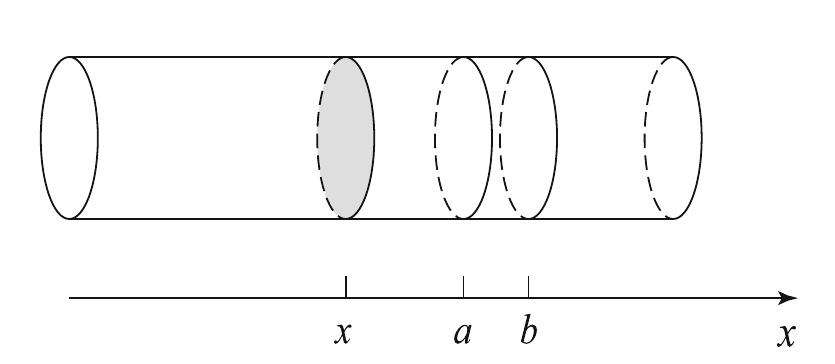
\includegraphics[scale=0.5]{images/cilindro01.png}
    \caption{Cilindro en el que fluye una masa de gas, en x hay una sección transversal}
    \label{fig:cilindro01}
\end{figure}

Si suponemos que las paredes del cilindro son impermeables para el gas, y la masa del gas ni se crea ni se destruye
al interior del cilindro, entonces la masa en ésta sección unicamente puede cambiar debido al flujo del gas
del punto $a$ al punto $b$.

Ahora, supongamos que $v(x,t)$ es la velocidad del gas en el punto $x$ al tiempo $t$.  Entonces la 
velocidad del flujo o el flujo másico $\phi$ que pasa por éste punto estará dado por la ecuación 
\eqref{eq:flujo-masico}:
\begin{equation}\label{eq:flujo-masico}
    \phi(x,t) = \rho(x,t)v(x,t)
\end{equation}
Que tiene unidades dadas por la expresión \eqref{eq:unidades01}:
\begin{equation}\label{eq:unidades01}
    \left[\phi\right]=\frac{kg}{s} = \left[\rho\right]\left[v\right]= \frac{kg}{\cancel{cm}}\frac{\cancel{cm}}{s}
\end{equation}

Así el flujo másico tendrá unidades de kilogramos ''$kg$'' por segundo ''$s$'', es decir una medida de la 
cantidad de masa que pasa por cada segundo en un punto $x$ particular dentro del intervalo.

Debido a que el flujo másico tiene unidades de kilogramos por segundo, entonces podemos derivar la 
ecuación \eqref{eq:masatotal01} de donde obtenemos la razón de cambio de la masa en el intervalo
$[a,b]$, y así obtener la expresión \eqref{eq:cambio_masa}:
\begin{equation}\label{eq:cambio_masa}
    \frac{d u(x,t)}{dt} = \frac{d}{dt}\int_a^b\rho(x,t)dx=\overbrace{\rho(a,t)v(a,t)}^{masa\ que\ entra}
    -\underbrace{\rho(b,t)v(b,t)}_{masa\ que\ sale}
\end{equation}
Que se puede interpretar como que el cambio en la masa en un instante de tiempo, es igual a la cantidad 
de masa que entra, menos la cantidad de masa que sale del cilíndro. La ecuación \eqref{eq:cambio_masa}
es una forma \textbf{integral} de la ley de conservación de masa. 

Otra forma se puede obtener integrando la densidad pero ahora en un intervalo de tiempo, por ejemplo $t\in [t_1,t_2]$, suponiendo que $t_2>t_1$, escrito en términos de la masa en el tiempo $t_1$ y del flujo másico en cada frontera, en ese mismo periodo de tiempo  \eqref{eq:densidad_tiempo}:
\begin{equation}\label{eq:densidad_tiempo}
\begin{aligned}
\int_{a}^{b} \rho\left(x, t_{2}\right) d x=& \int_{a}^{b} \rho\left(x, t_{1}\right) d x \\
&+\int_{t_{1}}^{t_{2}} \rho\left(a, t\right) v\left(a, t\right) d t-\int_{t_{1}}^{t_{2}} \rho\left(b, t\right) v\left(b, t\right) d t .
\end{aligned}
\end{equation}
Para derivar la forma diferencial de la leyes de conservación, debemos asumir que 
tanto $\rho(x, t)$ como $v(x, t)$ son funciones diferenciables.  Entonces usando la expresión \eqref{eq:densidad_variable}:

\begin{equation}\label{eq:densidad_variable}
\rho\left(x, t_{2}\right)-\rho\left(x, t_{1}\right)=\int_{t_{1}}^{t_{2}} \frac{\partial}{\partial t} \rho(x, t) d t
\end{equation}
y que la diferencia en el flujo másico se puede escribir como \eqref{eq:flujo_masico_diff}: 
\begin{equation}\label{eq:flujo_masico_diff}
\rho\left(b, t\right) v\left(b, t\right)-\rho\left(a, t\right) v\left(a, t\right)=\int_{a}^{b} \frac{\partial}{\partial x}(\rho(x, t) v(x, t)) d x
\end{equation}
y reemplazando estas expresiones en \eqref{eq:densidad_tiempo}, se obtiene \eqref{eq:intdoble01}:
\begin{equation}\label{eq:intdoble01}
\int_{t_{1}}^{t_{2}} \int_{a}^{b}\left\{\frac{\partial}{\partial t} \rho(x, t)+\frac{\partial}{\partial x}(\rho(x, t) v(x, t))\right\} d x d t=0
\end{equation}
Puesto que esto debe cumplirse tanto en el intervalo  $x\in\left[a, b\right]$ y en el intervalo de tiempo $t\in\left[t_{1}, t_{2}\right]$, podemos concluir que el integrando en la expresión \eqref{eq:intdoble01} debe ser identicamente cero, obteniendo la forma diferencial de la ley de conservación de la masa \eqref{eq:ley_conservacion_masa_02}:
\begin{equation}\label{eq:ley_conservacion_masa_02}
\rho_{t}+(\rho v)_{x}=0 \quad \text { Ley diferencial de la conservación de la masa }
\end{equation}

\section{Casos especiales de las leyes de conservación}
A continuación presentamos algunos casos especiales de las leyes de conservación.

\section{Ejemplos de modelos matemáticos}


